\documentclass[letterpaper, 11pt]{article}

\usepackage{lastpage, siunitx, hyperref, amsmath, color, graphicx}

%\definecolor{orange}{rgb}{1,0.5,0}

\def\UrlBreaks{\do\/\do-}

%\usepackage[hyphens]{url}

\usepackage[margin=1in]{geometry}
%\geometry{hscale=.6, vscale=.8, hmarginratio=2:1, vmarginratio=1:1, marginparwidth=.18\paperwidth, ignoremp}
%\geometry{marginparwidth=.1\paperwidth}

%\usepackage[T1]{fontenc}

%\usepackage[explicit]{titlesec}
%\titlespacing*{\section}{\dimexpr -\marginparsep-\marginparwidth}{*4}{*1}
%\titleformat{\section}[runin]{\large\bfseries\titlerule[.5pt]\filright}{\makebox[1em][c]{\thesection}}{1em}{\parbox[t]{\dimexpr\marginparwidth-2em}{#1}\hskip\marginparsep\mbox{}}[\newline\vspace{-4ex}]

%\titlespacing*{\subsection}{\dimexpr -\marginparsep-\marginparwidth}{*4}{*1}
%\titleformat{\subsection}[runin]{\large\bfseries\titlerule[.5pt]\filright}{\makebox[1em][c]{\thesection}}{1em}{\parbox[t]{\dimexpr\marginparwidth-2em}{#1}\hskip\marginparsep\mbox{}}[\newline]

\usepackage{enumitem}
\newlist{steps}{enumerate}{1}
\setlist[steps]{label=Step \arabic*, font=\bfseries, leftmargin=-\marginparsep, itemindent=\marginparsep, align=right}

\usepackage{fancyhdr}
\pagestyle{fancy}
\fancyhf{}
%\fancyhfoffset[lh,lf]{\dimexpr\marginparwidth+\marginparsep}
\fancyhf[lh]{UCD EEC 134}
\fancyhf[ch]{}
\fancyhf[rh]{}
%\fancyhf[lf]{left foot}
%\fancyhf[cf]{centre foot}
\fancyhf[rf]{Page \thepage /\pageref{LastPage}}
%\renewcommand{\footrulewidth}{.4pt}

%%%%%%%%%%%%%%%
%%%% Tikz definitions
%%%%%%%%%%%%%%%
%\tikzstyle{Uno}=[rectangle,fill=white,draw,line width=0.5mm]

%new commands
%display due date in red and link to the eec134-schedule.pdf document
\newcommand{\due}[1]{\href{https://github.com/ucdart/UCD-EEC134/blob/master/support/schedule/eec134-schedule.pdf}{\textcolor{red}{#1}}}

\graphicspath{{./figures/}}

\begin{document}

\title{EEC 134 PCB 3 Guidelines}
\author{Instructor: Xiaoguang ``Leo'' Liu\\lxgliu@ucdavis.edu \\
	\small \href{http://creativecommons.org/licenses/by-sa/4.0/}{CC BY-SA 4.0}}
%\date{}
\date{Last updated: \today}

\maketitle

In Lab 3, we will start putting multiple RF components together on a single PCB to prepare you for your Quarter 2 design. In particular, you will design a simple transmitter PCB according to Fig.\ref{fig:pcb3}.

\begin{figure}[h]
	\centering
	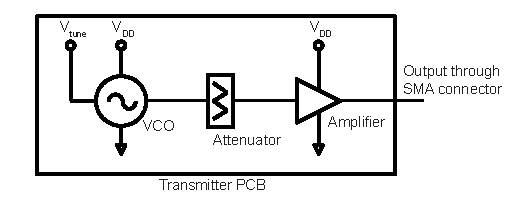
\includegraphics{blockdiagram.pdf}
	\caption{System block diagram for PCB 3.}
	\label{fig:pcb3}
\end{figure}

\section{Design Requirements}

\begin{itemize}
	\item The main components used in this design are 
		\begin{enumerate}
			\item VCO: Maxim MAX2750
			\item Attenuator: Analog Devices HMC653LP2E
			\item Amplifier: Analog Devices ADL5611
		\end{enumerate}
	\item Desired output frequency range: 2.3--2.5\,GHz
	\item Desired output power: $>$15\,dBm
	\item Output connector: SMA, same as in PCB 2. 
	\item The PCB should be less than 1"$\times$2" in size. The smaller the better. 
\end{itemize}

\section{Some tips}

\begin{enumerate}
	\item Read the datasheets of these components carefully to understand their characteristics. You should follow the manufacturer's recommended schematic and layout designs. If the manufacturer provides evaluation boards, see if you can obtain the designs files and use them as a reference.
	
	\item Make sure to include dc-blocking capacitors at the input and output of the active components to ensure that the components can be biased correctly. 
	
\end{enumerate}
 
\section{Test Report Requirements}
In the test report, please include the following
\begin{itemize}
	\item Circuit schematic 
	\item PCB layout 
	\item Measured output frequency vs $V_{tune}$
	\item Measured output power vs output frequency
	\item Discussion of the measured results. 	
\end{itemize}

\section{Critical Dates}

\begin{itemize}
	\item Mar. 1st, 2020: PCB 3 design and review report 
	\item Mar. 1st, 2020: PCB 3 design files 
	\item Mar. 19th, 2020: PCB 3 test reports
\end{itemize}

\end{document}